%%% UNIT 2
{
\setbeamertemplate{headline}{}
\setbeamertemplate{footline}{
  \begin{beamercolorbox}[wd=\paperwidth,ht=2.2ex,dp=1.5ex]{palette quaternary}
  \end{beamercolorbox}
  }
\begin{frame}[noframenumbering]
\frametitle{\DB{\huge{\textbf{$\blacksquare$ Unit 2}}}}
\myPause
 \begin{itemize}
 \item[] \LARGE{\MB{Feedback and its magic}}
 \item[] \vspace{-1mm}\LARGE{\MB{Dynamic systems}}
 \item[] \vspace{-1mm}\LARGE{\MB{The DT LTI case in detail}}
 \item[] \vspace{-1mm}\LARGE{\MB{Conclusions and discussion}}
 \end{itemize}
\end{frame}
}

\part{}

\section{Feedback (informally)}
\subsection{}

\begin{frame}\mccz
\frametitleTC{Feedback and its magic}
\myPause
 \begin{columns}
  \column[T]{0.45\textwidth}
   \only<2->{\centering
\includegraphics[height=6cm]{./Unit-02/img/Feedback-TheMagic_cc0.jpg}}\myPause%
  \column[T]{0.55\textwidth}
   \begin{itemize}[<+-| alert@+>]
   \item If PROPERLY used, feedback can
         \begin{itemize}[<+-| alert@+>]
         \item \vspace{2mm}counteract model errors\\
                and uncertainties,
         \item \vspace{2mm}reject a disturbance\\
                without the need\\
                for its measurement,
         \item \vspace{2mm}stabilise an unstable\\
               or ``runaway'' system.
         \end{itemize}
   \item \vspace{4mm}Let us see.
   \end{itemize}
 \end{columns}
\end{frame}

\begin{frame}
\frametitleTC{Feedback to counteract model errors/uncertainty and disturbances}
\framesubtitleTC{(to introduce this idea we do not use dynamic systems for simplicity)}
\myPause
 \begin{itemize}[<+-| alert@+>]
 \item \vspace{-8mm}Consider a controlled system such that the outcome $O$ depends on the control action $A$ and
       the disturbance $D$ as \textcolor{magenta}{$O=0.5(A+D)$.}
 \item If we want to use open-loop control and to make $O$ equal a reference $R$, we must solve for $A$ the equation
       $0.5(A+D)=R$, whence the control law \DG{$A=2R-D$.}
 \item Let us verify with some numbers:
 \item[] \begin{center}
          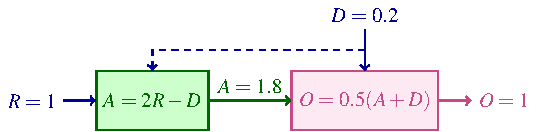
\includegraphics[width=0.60\columnwidth]{./Unit-02/img/Taxonomy-OpenLoop-Example-FullKnowledge.pdf}
          \hspace{6mm}
\includegraphics[height=1.5cm]{./Unit-02/img/smile.png}
         \end{center}
 \end{itemize}
\end{frame}

\begin{frame}
\frametitleTC{Feedback to counteract model errors/uncertainty and disturbances}
\myPause
 \begin{itemize}[<+-| alert@+>]
 \item But what if we assume \textcolor{magenta}{$O=0.5(A+D)$} while the true system is
       \textcolor{magenta}{ $O=\mathbf{0.6}(A+D)$}?
 \item If we use the nominal control law \DG{$A=2D-R$} on the true system, we get the following:
 \item[] \begin{center}
          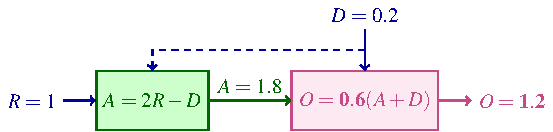
\includegraphics[width=0.65\columnwidth]{./Unit-02/img/Taxonomy-OpenLoop-Example-PartialKnowledge.pdf}
          \hspace{6mm}
\includegraphics[height=1.5cm]{./Unit-02/img/frown.png}
         \end{center}
 \item \vfill H\'{e}las, 20\% error on a model parameter (0.6 instead of 0.5)\\
       $\Rightarrow$ 20\% error of $O$ wrt $R$.
 \item Open-loop control cannot counteract model errors.
 \item Let us try with feedback.
 \end{itemize}
\end{frame}

\begin{frame}
\frametitleTC{Feedback to counteract model errors/uncertainty and disturbances}
\myPause
 \begin{itemize}[<+-| alert@+>]
 \item \underline{EXAMPLE} feedback scheme with \TC{proportional} control (action $A$ proportional\\
       to the \TC{error} $R-O$); note that we do not compensate the disturbance:
 \item[] \begin{center}
          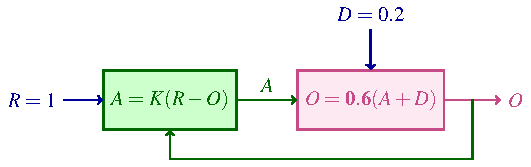
\includegraphics[width=0.60\columnwidth]{./Unit-02/img/Taxonomy-ClosedLoop-Example.pdf}
         \end{center}
 \item Joining the system and controller equations, for $O$ we get
       \begin{displaymath}
        \begin{array}{rcl}
         \left\{\begin{array}{rl}
          A &= K(R-O) \\
          O &= 0.6(A+D)
         \end{array}\right. &
         \Rightarrow &
          O = \frac{3K}{3K+5}R+\frac{3}{3K+5}D
         \end{array}
        \end{displaymath}
 \item Apparently, as $K \rightarrow \infty$, $O \rightarrow R$ $\forall D$.
 \item \vfill Yes, feedback can counteract model errors and disturbances;
 \item possible drawbacks on stability (improper use of feedback) later on. 
 \end{itemize}
\end{frame}

\begin{frame}
\frametitleTC{Studying the stability of a system}
\framesubtitleTC{adopting here a \underline{very} informal attitude, where ``stable'' means ``left alone, does not
                 run amok''}
\myPause
 \begin{itemize}[<+-| alert@+>]
 \item Let us take our system, initialise $y(0)$ to $y_0$, let $u(k)=0$ $\forall k$ so that
       \begin{displaymath}
        y(k) = ay(k-1),
       \end{displaymath}
       and see what happens.
 \item \vfill Case 1: $|a|<1$, for example 0.5 or -0.5.\\
 \item[] For $k=0,1,2,\ldots$, we have respectively the $y$ sequences
       \begin{displaymath}
        \begin{matrix*}[r]
          y_0, &  0.5y_0, & 0.25y_0, &  0.125y_0, \ldots \\
          y_0, & -0.5y_0, & 0.25y_0, & -0.125y_0, \ldots
        \end{matrix*}
       \end{displaymath}       
 \item[] For $k\rightarrow\infty$ the system's \TC{free motion} (no input) converges to zero\\
         $\Rightarrow$ we say the system is \TC{asymptotically stable.}      
 \end{itemize}
\end{frame}

\begin{frame}
\frametitleTC{Studying the stability of a system}
\myPause
 \begin{itemize}[<+-| alert@+>]
 \item Case 2: $|a|=1$, i.e., $a=\pm 1$.\\
 \item[] For $k=0,1,2,\ldots$, we have respectively the $y$ sequences
       \begin{displaymath}
        \begin{matrix*}[r]
          y_0, &  y_0, & y_0, &  y_0, \ldots \\
          y_0, & -y_0, & y_0, & -y_0, \ldots
        \end{matrix*}
       \end{displaymath}       
 \item[] For $k\rightarrow\infty$ the free motion neither converges to zero nor diverges\\
         $\Rightarrow$ we say the system is \TC{stable}, but not asymptotically.
 \item \vfill Case 3: $|a|>1$, for example 2 or -2.\\
 \item[] For $k=0,1,2,\ldots$, we have respectively the $y$ sequences
       \begin{displaymath}
        \begin{matrix*}[r]
          y_0, &  2y_0, & 4y_0, &  8y_0, \ldots \\
          y_0, & -2y_0, & 4y_0, & -8y_0, \ldots
        \end{matrix*}
       \end{displaymath}
 \item[] For $k\rightarrow\infty$ the free motion diverges (except for the one case $y_0=0$)\\
         $\Rightarrow$ we say the system is \TC{unstable.} 
 \end{itemize}
\end{frame}


\begin{frame}
\frametitleTC{Stabilising a system by means of feedback}
\myPause
 \begin{itemize}[<+-| alert@+>]
 \item Take an unstable system:
       \begin{displaymath}
        y(k) = ay(k-1)+u(k-1), \qquad a=2.
       \end{displaymath}
 \item Feed $y$ back to $u$ proportionally, i.e., set $u(k) = Qy(k)$.
 \item Doing so we have the closed-loop system
       \begin{displaymath}
        y(k) = 2y(k-1)+Qy(k-1) = (2+Q)y(k-1)
       \end{displaymath}
       and if we chose $Q$ so that $|2+Q|<1$, this is asymptotically stable.
 \end{itemize}
\end{frame}

\begin{frame}
\frametitleTC{Stabilising a system by means of feedback}
\framesubtitleTC{and once again, tolerating model errors/uncertainties}
\myPause
 \begin{itemize}[<+-| alert@+>]
 \item Note that feedback control is also naturally \TC{robust} (for the moment,\\
       think of this as ``resilient to model errors'').
 \item For example, take $Q=-1.5$ so that $2+Q=0.5$.
 \item In this case the closed loop is asymptotically stable not only for $a=2$,\\
       but $\forall a$ s.t. $|a+Q|=|a-1.5|<1$, i.e., for $0.5<a<2.5$.
 \item \vspace{4mm} Summing up, with feedback we can impose stability even if we do not know\\
       the system (here, parameter $a$) precisely...
 \item[]\vspace{-1mm} ...but for the very same reasons, we might also \emph{destroy} stability.
 \item Feedback is a powerful weapon, use with care.
 \item \vfill And now, let us re-address feedback and dynamic systems\\
       with a formal attitude (soon focusing on the DT LTI case).
 \end{itemize}
\end{frame}



\section{Dynamics (formally)}
\subsection{}

\begin{frame}
\frametitleTC{System -- recap and systematisation}
\framesubtitleTC{A mathematical representation (model) of something that evolves}
\myPause
 \begin{columns}
  \column[T]{0.45\textwidth}
   \begin{itemize}[<+-| alert@+>]
   \item[] Simple representation
   \item[] \vspace{2mm}\begin{center}
            \usetikzlibrary{matrix}
\usetikzlibrary{arrows}
\usetikzlibrary{calc}

\tikzstyle{block} = [draw,rectangle,thick,minimum height=3em,minimum width=4em]
\tikzstyle{sum} = [draw,circle,inner sep=0mm,minimum size=2mm]
\tikzstyle{connector} = [->,thick]

\begin{tikzpicture}[scale=1.00]

\node [left] at (00.00,00.00) (in_u) {$u$};
\node [block] at (01.20,00.00) (S) {{\huge$\mathcal{S}$}};
\draw [connector] (in_u.east) -- (S.west);
\node [right] at (02.40,00.00) (out_y) {$y$};
\draw [connector] (S.east) -- (out_y.west);
\end{tikzpicture}


           \end{center}
           \begin{itemize}[<+-| alert@+>]
           \item[] $u$ -- input(s)
           \item[] $y$ -- output(s)
           \end{itemize}
   \end{itemize}
  \column[T]{0.55\textwidth}
   \begin{itemize}[<+-| alert@+>]
   \item[] Model ingredients
           \begin{itemize}[<+-| alert@+>]
           \item what the system evolves upon:
                 \begin{itemize}[<+-| alert@+>]
                 \item the \TC{continuous time} $t$;
                 \item an integer index $k$ counting some events,
                       frequently called\\the \TC{discrete time}.
                 \end{itemize}
           \item the \TC{evolution law}:
                 \begin{itemize}[<+-| alert@+>]
                 \item $u[t_0,t]\;\rightarrow\;y[t_0,t]$;
                 \item $u[k_0,k]\;\rightarrow\;y[k_0,k]$.
                 \end{itemize}
           \end{itemize}
   \end{itemize}
 \end{columns} \myPause
 \vfill
 \begin{center}
  \vfill \textbf{Is anything missing? \myPause Sometimes, yes.}
 \end{center}
\end{frame}

\begin{frame}
\frametitleTC{\underline{Dynamic} system -- recap and systematisation}
\framesubtitleTC{The most general definition}
\myPause
\begin{center}
 {\Large
 If the knowledge of $u[t_0,t]$ --- or $u[k_0,k]$ \\ \myPause
 allows to determine $y[t_0,t]$ --- or $y[k_0,k]$ \\ \myPause
 the system is said to be \TC{non dynamic},\\ \myPause
 \vspace{1.5mm}\TC{dynamic} otherwise. \myPause
 }
\end{center}
\end{frame}

\begin{frame}
\frametitleTC{Dynamic system -- recap and systematisation}
\framesubtitleTC{Input, output, and \emph{state}}
\myPause
\begin{itemize}[<+-| alert@+>]
\item Non dynamic system:\\
      $y[t_0,t]$ or $y[k_0,k]$ depends only on $u[t_0,t]$ or $u[k_0,k]$.
\item Dynamic system:\\
      $y[t_0,t]$ or $y[k_0,k]$ depends on $u[t_0,t]$ or $u[k_0,k]$,\\
      and on the initial values $x[t_0]$ or $x[k_0]$ of some quantities.
\item These are called the \TC{state variables}, and form the \TC{state (vector)}.
\item The number of state variables is called the \TC{order} of the system.
\end{itemize}
\end{frame}

\begin{frame}
\frametitleTC{Dynamic system -- recap and systematisation}
\framesubtitleTC{How can we express this in mathematical terms?}
\myPause
In several ways. We see the only two relevant for us.\myPause
\begin{itemize}[<+-| alert@+>]
\item Continuous-Time (CT) system:\\
      \begin{displaymath}
       \left\{
        \begin{array}{rl}
         \frac{dx(t)}{dt} &= f \big( x(t),u(t),t  \big) \\
         y(t)             &= g \big( x(t),u(t),t  \big)
        \end{array}
       \right.
      \end{displaymath}
\item Discrete-Time (DT) system:\\
      \begin{displaymath}
       \left\{
        \begin{array}{rl}
         x(k) &= f \big( x(k-1),u(k-1),k  \big) \\
         y(k) &= g \big( x(k),u(k),k  \big)
        \end{array}
       \right.
      \end{displaymath}

\end{itemize}
\end{frame}

\begin{frame}
\frametitleTC{Dynamic system -- recap and systematisation}
\framesubtitleTC{Some more definitions (for both the CT and the DT case)}
\myPause
\begin{itemize}[<+-| alert@+>]
\item \TC{Linear (L)} system:\\
      $f(\cdot,\cdot,\cdot)$ and $g(\cdot,\cdot,\cdot)$ linear in $x$ and $u$.
\item \TC{Time-Invariant (TI)} system:\\
      $f(\cdot,\cdot,\cdot)$ and $g(\cdot,\cdot,\cdot)$ not depending on $t$ or $k$.
\item \TC{Proper} (sometimes, \emph{strictly} proper) system:\\
      $g(\cdot,\cdot,\cdot)$ not depending on $x$,\\
      i.e., the input acts on the output only through the state.
\item \TC{SISO} (Single-Input, Single-Output) system:\\
      $u$ and $y$ -- not necessarily $x$ -- scalars.
\end{itemize}
\end{frame}

\begin{frame}
\frametitleTC{Motion}
\framesubtitleTC{General definition}
\myPause
\centerline{Note: from now on we mostly speak DT, for CT just replace $k$ with $t$.} \myPause
\vspace{3mm}\begin{itemize}[<+-| alert@+>]
\item Initial state + input at a certain start time $\Rightarrow$ motion, i.e.,
      \begin{displaymath}
       \left.
        \begin{array}{l}
         x(k_0) \\ u(k),\,k \geq k_0
        \end{array}
       \right\}
       \quad \Rightarrow \quad
        x(k),y(k),\,k \geq k_0.
      \end{displaymath}
\item We call $x(k)$ and $y(k)$, respectively,
      \begin{itemize}[<+-| alert@+>]
      \item the \TC{state motion}
      \item and the \TC{output motion}
      \end{itemize}
\item [] produced by the initial state $x(k_0)$ and the input $u(k)$, starting\\
      at time $k_0$.
\end{itemize}
\end{frame}

\begin{frame}
\frametitleTC{Motion}
\framesubtitleTC{for the Time-Invariant (TI) case, to which we restrict the scope from now on}
\myPause
\begin{itemize}[<+-| alert@+>]
\item Initial state + input $\Rightarrow$ motion independently of the start time, i.e.,
      \begin{displaymath}
       \left.
        \begin{array}{l}
         x(0) \\ u(k),\,k \geq 0
        \end{array}
       \right\}
       \quad \Rightarrow \quad
        x(k),y(k),\,k \geq 0.
      \end{displaymath}
\item Alternatively, we can say that with TI systems one can set the origin\\
      of the time axis wherever one wants (for convenience, at zero).
\end{itemize}
\end{frame}

\begin{frame}
\frametitleTC{Equilibrium}
\framesubtitleTC{Definition (in the TI case)}
\myPause
\begin{center}
 {\Large
 If there exist some state vectors $\overline{x}$\\ \myPause
 such that $x(0)=\overline{x}$ and $u(k)=\overline{u}$, $k \geq 0$,\\ \myPause
 produce the constant state motion $x(k)=\overline{x}$, $k \geq 0$,\\ \myPause
 then those vectors are called \TC{equilibrium states},\\ \myPause
 or \TC{equilibria} for short,\\ \myPause
 \vspace{1.5mm}corresponding to the constant input $\overline{u}$.
 }
\end{center}
\end{frame}


\begin{frame}
\frametitleTC{Equilibrium}
\framesubtitleTC{Finding equilibrium states and outputs}
\myPause
\begin{itemize}[<+-| alert@+>]
\item A state vector $\overline{x}$ is an equilibrium for a given $\overline{u}$ if the consequent motion is
      $x(k)=x(k-1)=\overline{x}$ $\forall k$.
\item Thus to find equilibria one solves
      \begin{displaymath}
       \overline{x} = f(\overline{x},\overline{u}).
      \end{displaymath}
\item If some equilibrium state exists, and $g(\overline{x},\overline{u})$ does not lose significance,\\
      the result is the corresponding \TC{equilibrium output} $\overline{y}$.
\end{itemize}
\end{frame}

\begin{frame}
\frametitleTC{Stability}
\framesubtitleTC{Preliminaries}
\myPause
\begin{itemize}[<+-| alert@+>]
\item The existence of an equilibrium implies NOTHING on what happens if the system does not start exactly
      at the equilibrium.
\item Discussing this is a matter of \TC{stability}.
\item One can talk about stability of equilibria, motions, and sometimes systems.
\item We define stability for an equilibrium, do not talk about motions,\\
      and move to systems later on.
\end{itemize}
\end{frame}

\begin{frame}
\frametitleTC{Stability}
\framesubtitleTC{Stable equilibrium}
\myPause
\begin{itemize}[<+-| alert@+>]
\item Let $\overline{x}$ be an equilibrium for the constant input $\overline{u}$.
\item Denote by $x_{\Delta}(k)$ the \TC{perturbed motion} produced by
      \begin{itemize}[<+-| alert@+>]
      \item the input $\overline{u}$,
      \item and the \TC{perturbed initial state} $x(0)=\overline{x}+\Delta\overline{x}$.
      \end{itemize}
\item Not that in general, $x_{\Delta}(k)$ will not be constant.
\item Denote by $||x||$ the norm (think here of the Euclidean norm)\\
      of vector $x$.
\end{itemize}
\end{frame}


\begin{frame}
\frametitleTC{Stability}
\framesubtitleTC{Stable equilibrium}
\myPause
\begin{itemize}[<+-| alert@+>]
\item An equilibrium $\overline{x}$ corresponding to the constant input $\overline{u}$ is said to be \TC{stable} if
      \begin{displaymath}
       \forall \varepsilon>0 \;
       \exists \delta_{\varepsilon}>0 \; : \;
       ||\Delta\overline{x}||<\delta_{\varepsilon}
       \Rightarrow ||x_{\Delta}(k)-\overline{x}||<\varepsilon \; \forall k \geq 0.
      \end{displaymath}
\item Interpretation: stable equilibrium means that
      \begin{itemize}[<+-| alert@+>]
      \item no matter how close one wants the \TC{entire} perturbed motion to remain to the equilibrium,
      \item a maximum distance of the initial state from the equilibrium can be\\
            found, that fulfils the desire.
      \end{itemize}
      \item Graphically,
            \begin{center}
             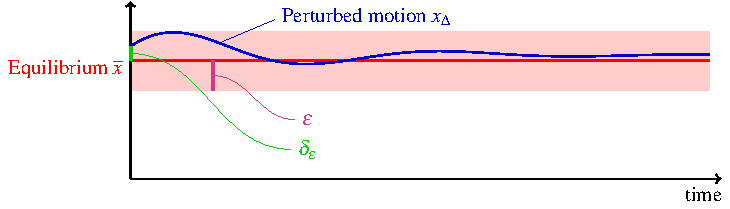
\includegraphics[width=0.60\columnwidth]{./Unit-02/img/StableEq-general.pdf}
            \end{center}
\item If the above does not hold true, the equilibrium is \TC{unstable}.
\end{itemize}
\end{frame}

\begin{frame}
\frametitleTC{Stability}
\framesubtitleTC{Asymptotically stable equilibrium}
\myPause
\begin{itemize}[<+-| alert@+>]
\item An equilibrium $\overline{x}$ corresponding to $\overline{u}$ is said to be \TC{asymptotically stable} if
      \begin{itemize}[<+-| alert@+>]
      \item it is stable,
      \item and \underline{in addition}
            \begin{displaymath}
             \lim_{k\rightarrow\infty} ||x_{\Delta}(k)-\overline{x}||=0.
            \end{displaymath}
      \end{itemize}
      \item Graphically,
            \begin{center}
             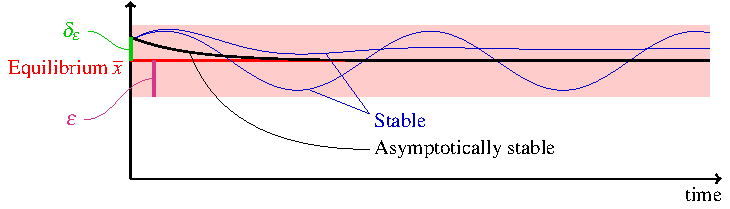
\includegraphics[width=0.60\columnwidth]{./Unit-02/img/AsympStableEq-general.pdf}
            \end{center}
\item Clearly asymptotic stability implies stability, but not \emph{vice versa}.
\end{itemize}
\end{frame}


\section{DT LTI -- state space}

\subsection{}

\begin{frame}
\frametitleTC{The DT LTI class}
\framesubtitleTC{Preliminaries}
\begin{itemize}[<+-| alert@+>]
\item For the LTI class, that we see here almost exclusively in the DT context, there exists a very strong theory.
\item The same is not true for more general (e.g., nonlinear) system classes.
\item Therefore, control problems of the type addressed here, are cast in the LTI framework wherever possible.
\item \vfill This motivates the importance of the DT LTI class, which we now\\
      come to examine.
\end{itemize}
\end{frame}

\begin{frame}
\frametitleTC{State-space representation of a DT LTI system}
\framesubtitleTC{Definition --- we stick to the SISO case for simplicity}
\myPause
\begin{itemize}[<+-| alert@+>]
\item The \TC{State-Space (SS)} representation of a DT LTI dynamic system is the quadruplet $(A,b,c,d)$ in
      \begin{displaymath}
       \left\{
        \begin{array}{rlll}
         x(k) &= A x(k-1) + b u(k-1) & & \text{\TC{(state equation)}}  \\
         y(k) &= c x(k)   + d u(k)   & & \text{\TC{(output equation)}}
        \end{array}
       \right.
      \end{displaymath}    
\item $u(k)$ and $y(k)$ are real scalars;
\item $x(k) \in \Re^n$, where $n$ is the system's order;
\item the real \TC{dynamic matrix} $A$ is $n \times n$;
\item $b$ is a real column vector ($n \times 1$);
\item $c$ is a real row vector ($1 \times n$);
\item $d$ is a real scalar.
\end{itemize}
\end{frame}

\begin{frame}
\frametitleTC{Motion}
\framesubtitleTC{}
\myPause
\begin{itemize}[<+-| alert@+>]
\item Given $x(0)$ and $u(k)$, $k \geq 0$, we get
      {\small
      \begin{displaymath}
       \begin{array}{rclcl}
        x(1) &=& Ax(0)+bu(0) \\
        x(2) &=& Ax(1)+bu(1) &=& A^2x(0)+Abu(0)+bu(1) \\
        x(3) &=& Ax(2)+bu(2) &=& A^3x(0)+A^2bu(0)+Abu(1)+bu(2) \\
             & & \cdots\\
       \end{array}
      \end{displaymath}
      }
\item This readily generalises to the \TC{Lagrange state formula}
      \begin{displaymath}
       x(k) = A^k x(0) +\sum\limits_{h=0}^{k-1} A^{k-h-1}bu(h).
      \end{displaymath}
\end{itemize}
\end{frame}

\begin{frame}
\frametitleTC{Free and induced state motion}
\framesubtitleTC{}
\myPause
\begin{itemize}[<+-| alert@+>]
\item In LTI systems, the state motion $x(k)$ is the \TC{sum} of a \TC{free motion} $x_F(k)$ and an
      \TC{induced motion} $x_I(k)$, i.e.,
      \begin{displaymath}
       x(k) = x_F(k) + x_I(k),
      \end{displaymath} \myPause
      where
      \begin{displaymath}
       x_F(k) = A^k x(0), \quad
       x_I(k) = \sum\limits_{h=0}^{k-1} A^{k-h-1}bu(h).
      \end{displaymath} \myPause
\item $x_F(k)$ depends linearly on $x(0)$ and not on $u$,
\item while $x_I(k)$ depends linearly only on $u(k)$ and not on $x(0)$.
\end{itemize}
\end{frame}

\begin{frame}
\frametitleTC{Free and induced output motion}
\framesubtitleTC{}
\myPause
\begin{itemize}[<+-| alert@+>]
\item In LTI systems, also the state motion $y(k)$ is the \TC{sum} of a \TC{free motion} $y_F(k)$ and an
      \TC{induced motion} $y_I(k)$, i.e.,
      \begin{displaymath}
       y(k) = y_F(k) + y_I(k),
      \end{displaymath} \myPause
      where
      \begin{displaymath}
       y_F(k) = cA^k x(0), \quad
       y_I(k) = c\sum\limits_{h=0}^{k-1} A^{k-h-1}bu(h) +du(k).
      \end{displaymath} \myPause
\item again, $y_F(k)$ depends linearly on $x(0)$ and not on $u$,
\item while $y_I(k)$ depends linearly only on $u(k)$ and not on $x(0)$.
\end{itemize}
\end{frame}

\begin{frame}
\frametitleTC{Equilibrium}
\framesubtitleTC{}
\myPause
\begin{itemize}[<+-| alert@+>]
\item For an LTI system, equilibrium states are found by solving
      \begin{displaymath}
       \overline{x} = A\overline{x}+b\overline{u}.
      \end{displaymath}
\item Thus, if $A$ has no unity eigenvalues, there exists the one equilibrium
      \begin{displaymath}
       \overline{x} = (I-A)^{-1}b\overline{u},
      \end{displaymath}
\item while in the opposite case, either there is no equilibrium, or there\\
      are infinite ones.
\end{itemize}
\end{frame}

\begin{frame}
\frametitleTC{Equilibrium}
\framesubtitleTC{Peculiarities of L(TI) systems}
\myPause
\begin{itemize}[<+-| alert@+>]
\item Contrary to nonlinear systems, they cannot have a finite number of equilibria, different from zero and one.
\item If some $\overline{u}$ produces zero, one or infinite equilibria, the same is true for any other $\overline{u}$,
      contrary again to the nonlinear case.
\item For each equilibrium state, there surely exists the one equilibrium output
      \begin{displaymath}
       \overline{y}=c\overline{x}+d\overline{u}.
      \end{displaymath}
\end{itemize}
\end{frame}

\begin{frame}
\frametitleTC{Stability of an equilibrium}
\framesubtitleTC{}
\myPause
\begin{itemize}[<+-| alert@+>]
\item Let $(\overline{x},\overline{u})$ be an equilibrium for an LTI system. 
\item The Lagrange state formula leads to write
      \begin{displaymath}
       \overline{x} = A^k \overline{x} +\sum\limits_{h=0}^{k-1} A^{k-h-1}b\overline{u}.
      \end{displaymath}.
\item Consider now the  perturbed motion $x_{\Delta}(k)$ produced by $\overline{u}$ and
      $x(0)=\overline{x}+\Delta\overline{x}$; the same formula yields
      \begin{displaymath}
       x_{\Delta}(k) = A^k (\overline{x}+\Delta\overline{x}) +\sum\limits_{h=0}^{k-1} A^{k-h-1}b\overline{u}.
      \end{displaymath}
\item Subtracting, therefore,
      \begin{displaymath}
       x_{\Delta}(k)-\overline{x} = A^k\Delta\overline{x}
      \end{displaymath}
\end{itemize}
\end{frame}

\begin{frame}
\frametitleTC{Stability of an equilibrium}
\framesubtitleTC{and in the L(TI) case, of a system}
\myPause
\begin{itemize}[<+-| alert@+>]
\item The way $x_{\Delta}(k)$ moves with respect to $\overline{x}$ does not depend on $\overline{x}$.
\item That is, contrary the nonlinear case, there cannot be equilibria with different stability characteristics.
\item In the L(TI) class, stability is a property of the \emph{system}, not of the individual equilibria.
\item Moreover, 
      \begin{itemize}[<+-| alert@+>]
      \item for $k\rightarrow\infty$, $||x_{\Delta}(k)-\overline{x}|| \rightarrow 0 \, \forall x(0)$  iff $A^k$
            converges to a zero matrix,
      \item the same norm generally diverges if at least one element of $A^k$ does,
      \item and if $A^k$ neither converges to zero nor diverges, the same happens\\
            to $||x_{\Delta}(k)-\overline{x}||$.
      \end{itemize}
\item Thus, in the LTI case, the stability of a system only depends on its\\
      dynamic matrix $A$.
\end{itemize}
\end{frame}

\begin{frame}[label={pag:stab-eivals}]
\frametitleTC{Stability and eigenvalues of $A$}
\framesubtitleTC{}
\myPause
\begin{itemize}[<+-| alert@+>]
\item The following can be proven.
      \begin{itemize}[<+-| alert@+>]
      \item An LTI system is asymptotically stable iff all the eigenvalues of $A$ have magnitude less  than one
            (or, equivalently, lie in the open \TC{unit circle} of the complex plane).
      \item The same system is unstable if (but not only if) at least one eigenvalue of $A$ has magnitude greater
            than one.
      \item If all the eigenvalues of $A$ have magnitude less than or equal to one, and there exists at least one
            with unity magnitude, the system can be either unstable\\
            or stable, but not asymptotically.
      \end{itemize}
\end{itemize}
\end{frame}

\begin{frame}
\frametitleTC{Properties of asymptotically stable systems}
\framesubtitleTC{also in a view to control}
\myPause
\begin{itemize}[<+-| alert@+>]
\item An asymptotically stable system has one and only one equilibrium for each constant input.
\item The state and output free motions of an asymptotically stable system converge to zero (norm)
      for $k\rightarrow\infty$.
\item As a consequence, asymptotically stable systems ``forget their initial condition''...
\item ...which is a definitely desired property for a \TC{controlled} system.
\end{itemize}
\end{frame}


\section{DT LTI -- transfer function and block diagrams}

\subsection{}

\begin{frame}
\frametitleTC{Preliminary}
\framesubtitleTC{for an alternative system representation, particularly useful for control}
\myPause
 \begin{itemize}[<+-| alert@+>]
 \item Let us introduce the \TC{one-step advance operator} $z$:
       \begin{displaymath}
        z\nu(k) := \nu(k+1) \qquad\qquad \text{whatever $\nu$ is}.
       \end{displaymath}
 \item This allows for a compact way to write LTI systems without evidencing the state (but it is there!).
 \item Suppose for example that we have a system with input $u$ and output $y$, ruled by
       \begin{displaymath}
        y(k) = ay(k-1)+bu(k-1),
       \end{displaymath}
       where clearly the state is the previous value of $y$;
 \item we can re-write $y(k+1)=ay(k)+bu(k)$ in the form
       \begin{displaymath}
        (z-a)y(k) = bu(k).
       \end{displaymath}
 \end{itemize}
\end{frame}

\begin{frame}
\frametitleTC{Preliminary}
\framesubtitleTC{introducing the transfer function}
\myPause
 \begin{itemize}[<+-| alert@+>]
 \item Rearranging -- remember the \emph{operatorial} meaning of $z$ -- we get
       \begin{displaymath}
        y(k) = \frac{b}{z-a}u(k)
       \end{displaymath}
\item[] and we can define the \TC{Transfer Function (TF)} notation, that expresses the system\\
        as a compound operator built upon the elementary one $z$:
       \begin{itemize}[<+-| alert@+>]
       \item we write the system's transfer function $G(z)$ as
             \begin{displaymath}
               G(z) = \frac{b}{z-a},
             \end{displaymath}
       \item[] and in force of this
             \begin{displaymath}
              y(k) = G(z)u(k) \quad \text{means} \quad y(k) = ay(k-1)+bu(k-1).
             \end{displaymath}
       \end{itemize}
 \item \vfill May not look so useful at the moment, but you will see later on\\
       how handy transfer functions are to determine controllers.
 \end{itemize}
\end{frame}

\begin{frame}
\frametitleTC{State space representation and transfer function}
\framesubtitleTC{}
\myPause
 \begin{itemize}[<+-| alert@+>]
 \item Given the SS representation we saw, shift all times by one (which is legit as the system is TI):
       \begin{displaymath}
        \left\{
         \begin{array}{rlll}
          x(k+1) &= A x(k)   + b u(k)\\
          y(k+1) &= c x(k+1) + d u(k+1) 
         \end{array}
        \right.
       \end{displaymath} 
 \item Apply the advance operator:
       \begin{displaymath}
        \left\{
         \begin{array}{rl}
          \textcolor{red}{z}x(k) &= A x(k) + b u(k)\\
          \textcolor{red}{z}y(k) &= c \textcolor{red}{z}x(k) + d\textcolor{red}{z} u(k)
         \end{array}
        \right.
       \end{displaymath} 
 \item Drop useless $z$'s and rearrange ($I$ is identity matrix of dimension $n$):
       \begin{displaymath}
        \left\{
         \begin{array}{rl}
          (zI-A)x(k) &= b u(k)\\
          y(k)       &= c x(k) + d u(k)
         \end{array}
        \right.
       \end{displaymath} 
 \end{itemize}
\end{frame}

\begin{frame}
\frametitleTC{State space representation and transfer function}
\framesubtitleTC{once again, sticking to the SISO case}
\myPause
 \begin{itemize}[<+-| alert@+>]
 \item Solve state equation for $x(k)$:
       \begin{displaymath}
        x(k) = (zI-A)^{-1} b u(k)
       \end{displaymath} 
 \item Substitute into output equation and rearrange:
       \begin{displaymath}
        y(k) = \textcolor{red}
                         {\underbrace{\left[c(zI-A)^{-1} b +d \right]}
                                    _{\text{Transfer function } G(z)}
                         } \; u(k)
       \end{displaymath} 
 \item We then define the transfer function of the generic SISO DT LTI\\
       system $(A,b,c,d)$ as
       \begin{displaymath}
        G(z) = c(zI-A)^{-1} b +d.
       \end{displaymath} 
 \end{itemize}
\end{frame}

\begin{frame}
\frametitleTC{Block diagrams}
\framesubtitleTC{Preliminaries}
\myPause
\begin{itemize}[<+-| alert@+>]
\item Block diagrams (BDs) are a graphical formalism to represent dynamic systems, that we see here limited to the
      DT LTI class.
\item They are useful to study \TC{interconnected} systems, i.e., compounds of \TC{subsystems} (e.g., a controller
      and the controlled object).
\item Important \emph{caveat}, that we state right from the beginning:
      \begin{itemize}[<+-| alert@+>]
      \item    a BD MUST NOT BE CONFUSED with a flow diagram;
      \item [] although subsystems have inputs and outputs,
      \item [] their compound comes from assembling \TC{equations}.
      \end{itemize}
\end{itemize}
\end{frame}

\begin{frame}
\frametitleTC{Block diagram components}
\framesubtitleTC{Block and summation node}
\myPause
\begin{center}
 \begin{picture}(210,70)(0,0)
  \put(000,35){\vector(1,0){30}}
  \put(000,40){{\small $u(k)$}}
  \put(030,20){\framebox(50,30)
              {$G(z)$}
              }
  \put(080,35){\vector(1,0){30}}
  \put(090,40){{\small $y(k)$}}

  \put(175,35){\circle{10}}

  \put(175,70){\vector(0,-1){30}}
  \put(150,62){{\small $u_1(k)$}}
  \put(165,40){{\small $+$}}

  \put(140,35){\vector(1,0){30}}
  \put(140,40){{\small $u_2(k)$}}
  \put(162,27){{\small $-$}}

  \put(175,00){\vector(0,1){30}}
  \put(150,03){{\small $u_3(k)$}}
  \put(167,20){{\small $+$}}

  \put(180,35){\vector(1,0){30}}
  \put(190,40){{\small $y(k)$}}
\end{picture}

\end{center} \myPause
\begin{itemize}[<+-| alert@+>]
\item \TC{Block} (left):\\
      an LTI SISO system with the indicated transfer function -- in the shown\\
      example, the \TC{equation} $G(z)u(k)-y(k)=0$.
\item \TC{Summation node} (right):\\
      a summation expression -- in the shown example, the \TC{equation}
      $u_1(k)-u_2(k)+u_3(k)-y(k)=0$.
\end{itemize}
\end{frame}


\section{Conclusions}
\subsection{}

\begin{frame}
\frametitleTC{Conclusions}
\framesubtitleTC{Recap and lessons learnt (1/2)}
\myPause
 \begin{itemize}[<+-| alert@+>]
 \item We can characerise a dynamic system with \TC{time domain responses}.
 \item These refer to a certain \emph{stimulus} (we used impulse and step).
 \item Responses can be used also to stipulate \TC{control objectives}.
 \item A viable way to do so is to transform time domain deires into some desired
       closed-loop transfer function.
 \item This paves the way to the \TC{direct synthesis} technique.
 \end{itemize}
\end{frame}

\begin{frame}
\frametitleTC{Conclusions}
\framesubtitleTC{Recap and lessons learnt (2/2)}
\myPause
 \begin{itemize}[<+-| alert@+>]
 \item We have open issues, however.
       \begin{itemize}[<+-| alert@+>]
       \item Why impulse and step \emph{stimuli} are meaningful?
       \item How can we choose the target closed-loop transfer function?
       \item What are the limits and what is their origin?
       \end{itemize}
 \item \vfill These issues are very suited for addressing in a practice session,\\
       which is our next task.
 \item Please review your notes, next time ask questions if needed\\
       before we start.
 \end{itemize}
\end{frame}

\section{}
{
\setbeamertemplate{headline}{
  \begin{beamercolorbox}[wd=\paperwidth,ht=4.2ex,dp=1.5ex]{palette quaternary}
  \end{beamercolorbox}
  }
\setbeamertemplate{footline}{
  \begin{beamercolorbox}[wd=\paperwidth,ht=2.2ex,dp=1.5ex]{palette quaternary}
  \end{beamercolorbox}
  }
\begin{frame}[noframenumbering]
 \vspace{20mm}\Huge{Discussion open}
\end{frame}
}


